%\documentclass[aps,prl,twocolumn,nobibnotes]{revtex4}
\documentclass[aps,showpacs,twocolumn,nobibnotes]{revtex4}
%\documentclass[aps,preprint,showpacs,nobibnotes]{revtex4}
%\documentclass[aps,preprint,nobibnotes]{revtex}
\usepackage{graphics,graphicx,amsfonts,amsmath,amsbsy,amssymb,color}
\usepackage{bm}
\usepackage[a4paper,vmargin={20mm,20mm},hmargin={20mm,10mm}]{geometry}
%\usepackage{epic}
%\usepackage{mciteplus}
\usepackage{subfigure}
\usepackage{paralist}
\usepackage{vector}  % Allows "\bvec{}" and "\buvec{}" for "blackboard" style bold vectors in maths
\newcommand{\D}[1] {D_{\bf #1}}
\def \beq {\begin{eqnarray}}
\def \eeq {\end{eqnarray}}
\def \Schrodinger {{Schr\"{o}dinger }}
\def \Di {{D_{\bfi}}}
\def \Dj {{D_{\bfj}}}
\newcommand {\adag}[1] {{a_{#1}^\dagger}}
\def \bfj {{\bf j}}
\def \bfi {{\bf i}}
\def \rone {{\bvec{r}_1}}
\def \rtwo {{\bvec{r}_2}}
\def \mEh {{\textrm{mE}_{\textrm{h}}}}
\def \Eh {{\textrm{E}_{\textrm{h}}}}
\def \nadd {{n_a}}
\newcommand{\braket}[3] {{\langle #1 | #2 | #3 \rangle}}
\newcommand{\brket}[2] {{\langle #1 | #2 \rangle}}
\newcommand{\bra}{\ensuremath{\langle}}
\newcommand{\ket}{\ensuremath{\rangle}}
%\def \ham {{\bf H}}
\def \ham {{\hat{H}}}
%\def \Sz {{\hat{\textrm{S}_{\textrm{z}}}}}
\def \Sz {{\hat{S}_z}}
\newcommand{\rff}[1]{{Eq.~\eqref{#1}}}
\def \Pgen {{P_{\textrm{gen}}}}
\def \Carb {{\textrm{C}_{\textrm{2}}}}
\def \Hij {{H_{\bvec{i}\bvec{j}}}}
\def \Kii {{K_{\bvec{i}\bvec{i}}}}
\def \Kij {{K_{\bvec{i}\bvec{j}}}}

\begin{document}
\title{Spectral functions of correlated extended systems via quantum embedding}
\author{George~H.~Booth}
%\email{ghb24@cam.ac.uk}
\author{Garnet~Kin-Lic~Chan}  
\affiliation{Department of Chemistry, Frick Laboratory, Princeton University, Princeton, New Jersey 08544, USA}

\begin{abstract}
The density matrix embedding theory (DMET) was introduced recently, and displayed the ability to seamless embed strongly entangled ground-state wavefunctions
within an extended environment [PRL {\bf 109} 186404 (2012)].
%With similarities 
%to the dynamical mean-field method, a set of local sites are self-consistently correlated, but with an analytically constructable bath describing the
%coupling to the rest of the extended system. 
Despite many formal advantages in the analytic embedding, the method was restricted to static, ground-state properties.
Here, we generalize the concept of quantum embedding to introduce a frequency dependence and demonstrate accurate spectral functions at a tiny
computational cost. Through this quantum embedding of a local spectral function within a mean-field response over the whole system, 
a coupling of the delocalized excitations is captured through a small set of 
analytically constructed, and now frequency-dependent bath states. In contrast to dynamical mean-field theory, the resultant 
spectral functions are directly obtained on the real-frequency axis, with no bath discretization error, and allow for straightforward generalization both 
to impurity clusters and arbitrary electron perturbation operators. We demonstrate
the application of this method to the paramagnetic Hubbard model, where we believe that for the low-energy excitations, these results represent some of the most accurate 
zero temperature, thermodynamic limit spectral functions for the Hubbard model to date, as well as showing the trivial extension to two-particle Greens functions. 
This vastly extends the scope and applicability 
of the DMET method in condensed matter problems as a computationally tractable route to correlated spectral functions of extended systems.
\end{abstract}
\date{\today}
\maketitle

Dynamic correlation functions are directly probed in most spectroscopic methods, as well as other techniques such as scanning tunneling microscopy (STM), 
and correspond to many of the important transport, optical, magnetic and wider electronic structure properties of materials. 
As such, their accurate computational prediction is highly sought after within the materials science community. 
However, few robust approaches exist for strongly correlated problems\cite{Gali2013}. The difficulty is in simultaneously requiring both an accurate 
treatment of the electron correlations beyond mean-field or low-order perturbation theory for the ground state {\em and} excitation spectrum, as well as modeling 
a system of sufficient size to mimic the thermodynamic limit of bulk properties and not suffer spurious finite size effects. 
However in general, it is only mean-field electronic structure methods which are computationally cheap enough to access the required system
sizes, and so there is a pressing need for methods with mean-field scaling, which can account for the excitation spectrum in strongly correlated 
and entangled systems.

A general, zero-temperature dynamic correlation function can be defined in the frequency domain as
\begin{equation}
    G(\omega;{\hat A},{\hat V}) = \langle \Psi^{(0)} | {\hat A}^{\dagger} \frac{1}{\omega-(H-E_0)+i \eta} {\hat V} | \Psi^{(0)} \rangle , \label{eqn:intCorrFunc}
\end{equation}
with the one- and two-particle Greens functions defined with $V$ and $A$ being single annihilation/creation operators or neutral excitation
operators respectively, with appropriate time-ordering of the operators. Spectral quantities are then defined as $A(\omega)=-\frac{1}{\pi}\Im[G(\omega)]$,
where the spectral broadening is given by the small imaginary component of the energy, $\eta$, which regularizes the correlation function. The single particle
density of states is given by the spectral representation of the one-particle Greens function, experimentally measured within STM 
and (angle-resolved) photoemission spectroscopy. However, other spectral functions are also highly sought after, such as the two-hole propagator, 
probed with Auger spectroscopy\cite{Mona2013}, or the two-electron Greens function, a key descriptor in Raman spectroscopy, and in the 
mechanism of high-$T_c$ superconductivity\cite{Millis2012,Millis2013}.

One such method which has proved successful in obtaining strongly correlated spectral functions is dynamical mean-field theory (DMFT)\cite{Georges1992,Georges1996,Kotliar2006}. In 
DMFT, the central variable is the local, one-particle Greens function, which is self-consistently embedded within a non-interacting or 
mean-field Greens function over the system. This is mapped to an impurity problem, which is then solved via an `impurity solver', such as 
continuous-time quantum Monte Carlo (CT-QMC)\cite{Millis2006}. However, there are some formal drawbacks of the DMFT formulation. If CT-QMC is used as an 
impurity solver (or indeed general QMC methods used in isolation), then the spectral functions are obtained only on the imaginary frequency 
axis, requiring unstable analytic continuation onto the real frequency axis, which can wash out the subtle or sharp features of the 
spectra\cite{Thomas2011}. In addition, accessing low temperature regimes encounters technical challenges related to the Fermion sign problem.
Alternative solvers such as exact diagonalization suffer from bath discretization error in the spectra due to the 
representation of the continuous Weiss field (at all frequencies) by a finite number of bath sites. In addition, since DMFT
is formulated from the one-particle Greens function, alternative spectra such as the two-particle Greens function and optical spectra are 
not straightforward to obtain, formally requiring expensive vertex corrections to compute\cite{Millis2012}. Other methods to calculate 
spectra of correlated extended systems, such as the dynamical density matrix renormalization group\cite{Jeckelmann2004} or perturbative
methods\cite{Senechal2000} are restricted to certain correlation strengths, system sizes or spatial dimensions.

Here, we aim to circumvent these issues, by generalizing and extending the idea of quantum embedding of {\em states}, as introduced in 
Ref.~\onlinecite{Chan2012}. This is achieved by embedding a local correlation function defined over a set of `impurity' sites, within an 
analytic coupling to the rest of the delocalized excitation space. This is determined through the Schmidt decomposition of a mean-field 
response computed throughout the bulk system. This renders the spectra exact in the non-interacting and local excitation limits. 
Since the method is formulated in terms of a general response vector, it is also not restricted in the type or rank of perturbation 
operators that it can consider. Furthermore, since the analytic coupling is only defined for a given frequency (rather than all frequencies 
for DMFT), the entanglement bath for the spectra is compact and exactly represents the coupling defined by the global response function. This 
allows for large impurity clusters to be treated with small numbers of additional `bath' states, without discretization error in the coupling 
to the extended system, and direct evaluation of spectra on the real frequency axis. The approach will be demonstrated for the Hubbard model, 
defined by the Hamiltonian in the site basis as
\begin{equation}
H = -t \sum_{\langle ij \rangle, \sigma} (a_{i,\sigma}^{\dagger}a_{j,\sigma} + \text{\textnormal {h.c.}}) + U \sum_i (n_{i,\uparrow} - \frac{1}{2})(n_{i,\downarrow} - \frac{1}{2})  . \label{eqn:hub}
\end{equation}
This lattice model encapsulates many of the difficulties in the electronic structure of correlated materials, displaying correlation driven 
phase transitions in the thermodynamic limit, and is closely representative of many transition metal oxides\cite{Limelette2003}, including qualitative aspects 
of high-$T_c$ superconductivity\cite{Millis2013,Anderson87}. Where possible, we compare to one-dimensional exact results\cite{Lieb68,Ovchinni1970}, as 
well as large-scale DMFT calculations\cite{Go2009,Kotliar2008}, in addition to demonstrating spectra for the doped system and two-particle Greens functions.

\emph{Method.-} Within the analytic quantum embedding formalism introduced for the ground state with the DMET method (see 
Ref.~\onlinecite{Chan2012} and \onlinecite{Chan2013} for details), the coupling between the correlated `impurity' sites, $\{ |\alpha \rangle \}$, and the rest 
of the system is represented via the component of the Schmidt basis of a single Slater determinant, $|\phi^{(0)}\rangle$, which couples the impurity space to 
the `environment' space external to the impurity. This analytic coupling is represented by a one-electron space of the same dimension as 
the impurity size, and denoted the ground-state {\em bath}, $\{ |\beta \rangle \}$. This space then spans the exact entanglement of the 
impurity space to its environment, as defined by the original mean-field function over the entire extended lattice. The interacting Hamiltonian 
is then projected into this space, which is now independent of the total number of sites in the system, and solved to return a ground-state 
wavefunction, $|\Psi^{(0)} \rangle$, in the space of $\{ |\alpha \rangle \} \otimes \{ |\beta \rangle \} \otimes \text{\textnormal {det}} \{ | \mu \rangle \}$, where $\{ | \mu \rangle \}$ 
represents the space of one-electron functions in $|\phi^{(0)}\rangle$ which are uncoupled to the impurity cluster after its Schmidt decomposition. Along with the 
bath space, a self-consistency procedure designed to match the elements of the one-body reduced density matrix derived from $|\phi^{(0)}\rangle$ and $|\Psi^{(0)} \rangle$ over the impurity sites,
returns a one-electron interaction potential, $u$, which describes some of the longer-ranged correlation effects, and controls the effective number of electrons in the impurity cluster.

We now generalize this procedure for the construction of a set of now frequency-dependent bath states into which the interacting
spectral functions can be projected. These bath states define the embedding in the wider system, and are derived from
a response vector determined from a one-electron Hamiltonian, $h$, which spans the entire lattice.
The first-order response function across the lattice is constructed as,
\begin{equation}
|\phi^{(1)}(\omega) \rangle = \left[ \omega-(h-\varepsilon_0)+i\eta \right]^{-1} {\hat V} |\phi^{(0)}\rangle = 
    {\hat G_0}(\omega) {\hat V} |\phi^{(0)} \rangle  , \label{nonintGF}
\end{equation}
where $h = t + u$ is a static, one-electron Hamiltonian over the lattice, defined by the non-interacting part of the Hamiltonian 
in Eq.~\ref{eqn:hub}, and the interaction potential obtained from the ground-state self-consistency. 
Although this is a one-electron Hamiltonian, the inclusion of the interaction potential mimics many of the correlation features of the interacting Hamiltonian.
For simplicity, we restrict ourselves in this letter to the case of {\em local} spectral functions, where ${\hat V}$ and ${\hat A}$ are both closed operators
within the impurity space, although extensions to non-local perturbations will be detailed in a forthcoming paper. This means that both the operator 
${\hat V}$ and $|\phi^{(0)} \rangle$ are spanned by the original ground-state 
space of $\{ |\alpha \rangle \} \otimes \{ |\beta \rangle \} \otimes \text{\textnormal {det}} \{ | \mu \rangle \}$. The frequency-dependent coupling to the environment 
results from the ${\hat G_0}$ operator, and we now Schmidt decompose its action onto ${\hat V} |\phi^{(0)} \rangle$, in order to isolate 
the coupling at each frequency point between the environment and fully correlated space of impurity sites and ground-state bath (i.e. 
space of $\{|\alpha \rangle \} \oplus \{|\beta \rangle \} \equiv \{ | \gamma \rangle \}$). The space external to this to which the coupling is defined 
is denoted by $\{| n \rangle \}$, which contains $\{ | \mu \rangle \}$. We choose to partition the response into these spaces to ensure that at all 
frequencies, we span the correlated ground-state wavefunction, $|\Psi^{(0)} \rangle$.

The action of ${\hat G_0}(\omega){\hat V}$ on $|\phi^{(0)} \rangle$ can be easily found in the eigenbasis of $h$, $\{ |\chi_r \rangle ; \epsilon_r \}$, 
and rotated such that the operators act solely within the partitioned spaces. For instance, with ${\hat V}=a_{\alpha}$, 
\begin{equation}
    {\hat G_0}(\omega){\hat V} = \sum_{\gamma} X_{\gamma}(\omega) a_{\gamma} + \sum_{n} X_{n}(\omega) a_n  ,
\end{equation}
with
\begin{equation}
    X_n(\omega) = \sum_{r \in \text{\textnormal {occ}}} \frac{\langle n|\chi_r \rangle \langle \chi_r | a_{\alpha} | \phi^{(0)} \rangle}{\omega - \epsilon_r + i \eta}   .
%    X_n(\omega) = \sum_{r \in \text{\textnormal {occ}}} \frac{|n \rangle \langle n|\chi_r \rangle \langle \chi_r | a_{\alpha} | \phi^{(0)} \rangle}{\omega - \epsilon_r + i \eta}   .
\end{equation}
For a two-index perturbation such as ${\hat V}=a_{\alpha}^{\dagger}a_{\alpha}$, the action of operator on $|\phi^{(0)} \rangle$ can be similarly decomposed as,
\begin{align}
    {\hat G_0}(\omega){\hat V} =& \sum_{\gamma \gamma'} X_{\gamma \gamma'} a_{\gamma}^{\dagger} a_{\gamma'} + \sum_{n \gamma} X_{n \gamma} a_n^{\dagger} a_{\gamma} \nonumber\\ 
                               +& \sum_{\gamma n} X_{\gamma n} a_{\gamma}^{\dagger} a_{n}  + \sum_{n n'} X_{n n'} a_n^{\dagger} a_{n'}    .   \label{eqn:2elpert}
\end{align}
The frequency-dependent bath states representing the coupling are then formed from the action on the external part of the space, $\{| n \rangle \}$. For instance, in the 
operator defined by Eq.~\ref{eqn:2elpert}, the action over the external space can be written as a new operator,
\begin{equation}
    {\hat B}(\omega) = 1 + \sum_{n \gamma} X_{n \gamma}(\omega) a_n^{\dagger} + \sum_{\gamma n} X_{\gamma n}(\omega) a_{n} + \sum_{n n'} X_{n n'}(\omega) a_n^{\dagger} .   \label{eqn:B}
\end{equation}
This operator defines the space, \mbox{$\mathcal{K}(\omega)=\text{\textnormal {span}} \left[ \{|\alpha \rangle \} \otimes \{ |\beta \rangle \} \otimes {\hat B}(\omega) \text{\textnormal {det}} \{ | \mu \rangle \} \right]$}, into which the fully-interacting 
response equations are then projected. The original ground-state space is included as the unity part of ${\hat B}(\omega)$, and the other states represent 
the frequency-dependent, many-electron bath states, which span the $|\phi^{(1)}(\omega) \rangle$ wavefunction defined in Eq.~\ref{nonintGF}.
The fully interacting response, $|\Psi^{(1)}(\omega) \rangle$, is calculated from
\begin{equation}
    P \left[ \omega - (H-E_0) + i \eta \right] P | \Psi^{(1)}(\omega) \rangle = P {\hat V} P |\Psi^{(0)} \rangle   ,   \label{eqn:ExactResponse}
\end{equation}
where $P=|\mathcal{K}(\omega) \rangle \langle \mathcal{K}(\omega) |$ is defined as the projector into the basis $\mathcal{K}(\omega)$. 
$|\Psi^{(0)} \rangle$ can be reoptimized in this new basis, however this was found empirically not to qualitatively change results, and 
so $|\Psi^{(0)}\rangle$ and $E_0$ are taken to be the ground-state wavefunction and energy in the 
original $\{|\alpha \rangle \} \otimes \{ |\beta \rangle \} \otimes \text{\textnormal {det}} \{ | \mu \rangle \} $ space. 
Since we are currently only considering local perturbations,
the projectors on the right-hand side of Eq.~\ref{eqn:ExactResponse} are not necessary, but included for completeness.
This equation is then solved via an exact, iterative procedure to obtain $| \Psi^{(1)}(\omega) \rangle$, and the correlation function desired is obtained from 
$G(\omega;{\hat A},{\hat V})=\langle \Psi^{(0)} | {\hat A}^{\dagger} | \Psi^{(1)}(\omega) \rangle$.

The number of individual operators in ${\hat B}(\omega)$ which define the contracted bath states from the Schmidt decomposition 
of $|\phi^{(1)}(\omega) \rangle$, grow with increasing particle rank of ${\hat V}$. For ${\hat V}=a_{\alpha}$, as required for the single-particle Greens function,
there is only one additional operator in ${\hat B}(\omega)$, and therefore the resultant dimension of the many-electron space $\mathcal{K}(\omega)$ in 
which the interacting equations are solved, is only approximately twice as large as the corresponding ground state space. For two-particle functions,
as shown in Eq.~\ref{eqn:2elpert}, there are $4 \times \text{\textnormal {dim}}\{|\gamma \rangle \} + 1$ operators. The actual increase in the size of the Hilbert
space in practice compared to the ground state is generally much smaller than this after consideration of particle number symmetry and removal of linear
dependencies (the basis is not generally orthonormal and the overlap matrix is explicitly considered). However, the key point of the 
approach is that the analytic construction of the bath states is no more costly than the diagonalization of the one-particle Hamiltonian, $h$, and once the
fully interacting response equation is projected into this basis, there is no dependence on the size of the underlying lattice, rendering the method
truly mean-field scaling with the size of the system. 

It should be noted that since the basis spanned by $\mathcal{K}(\omega)$ includes within it the space of $|\phi^{(1)}(\omega) \rangle$ by construction, 
and since this response is exact in the non-interacting limit (since $h$ is also exact), $|\Psi^{(1)}(\omega)\rangle$ is similarly exact in this limit.
In addition, for uncoupled, local excitations of the impurity cluster, $|\Psi^{(1)}(\omega)\rangle$ is also exact, due to the completeness of the 
$|\alpha \rangle$ space included in $\mathcal{K}(\omega)$. It is now necessary to turn to numerical applications of the method to determine the
quality of the results away from these exact limits. 
In this letter, we restrict ourselves to consider the one- and two-electron local Greens function,
defining the local density of states, and the density-density spectral functions respectively, while other local dynamic correlation functions can be obtained analogously.
To underline the small cost at which these thermodynamic limit results were obtained, all calculations presented were achieved on a single computing core at a 
computational cost of at most a few seconds per frequency point.

%+++++++++++++++++++++++++++++++++++++++++++++++++++++++
%   1D HUBBARD MODEL PLOTS vs. CDMFT
%+++++++++++++++++++++++++++++++++++++++++++++++++++++++
\begin{figure}
\begin{center}
    \vspace{-2mm}
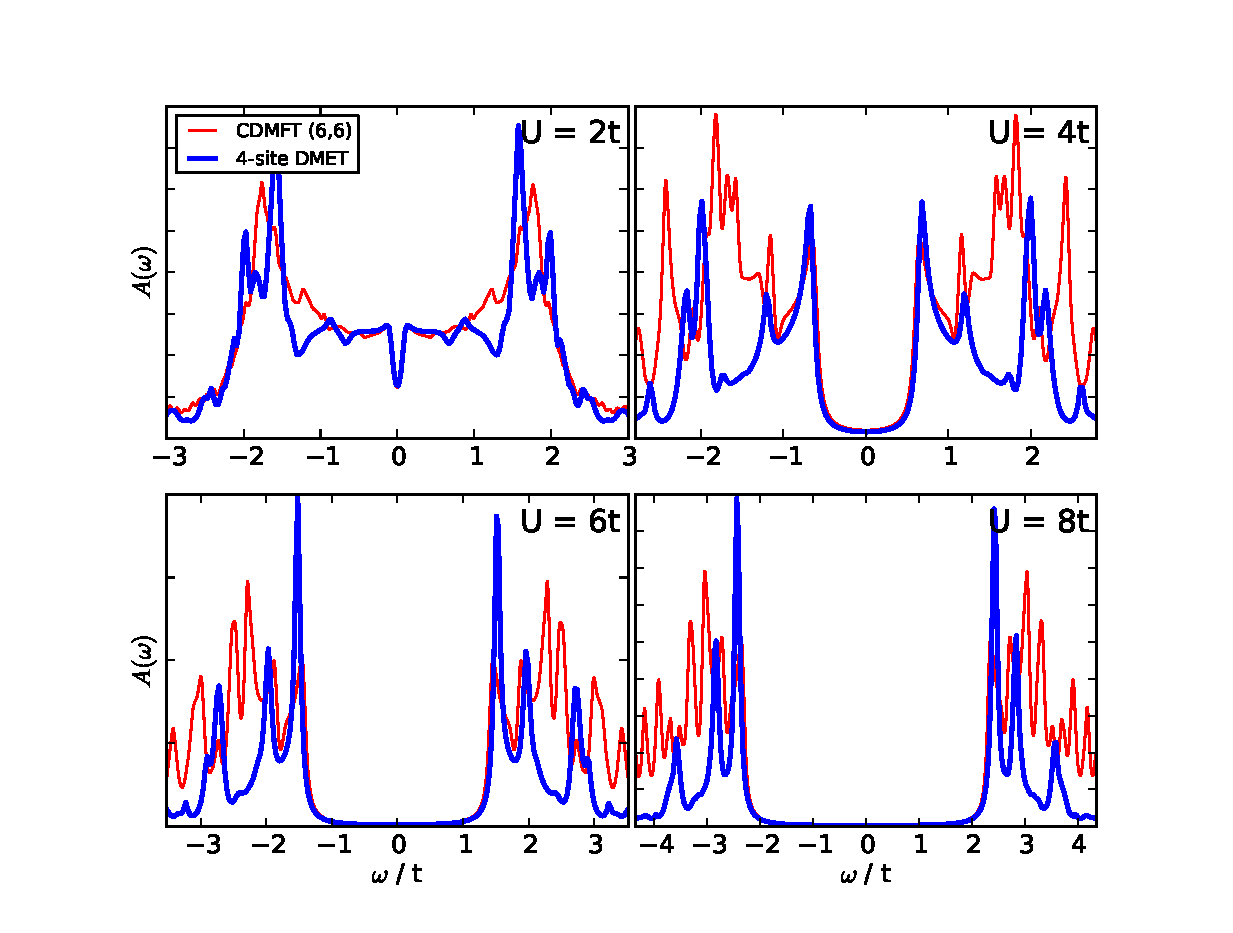
\includegraphics[scale=0.475]{Plots/1D_Spectra/1D_Hub_Spectra.eps}
\end{center}
    \vspace{-8mm}
\caption{Comparison of the local density of states between a four impurity cluster DMET calculation and a
(six impurity, six bath) CDMFT calculation for the half-filled 1D Hubbard model. The analytic bath construction
of DMET renders the spectral functions smooth over the frequency range.}
\label{1D_DOS}
\end{figure}

%+++++++++++++++++++++++++++++++++++++++++++++++++++++++
%   1D HUBBARD SPECTRAL GAP 
%+++++++++++++++++++++++++++++++++++++++++++++++++++++++
\begin{figure}
\begin{center}
    \vspace{-2mm}
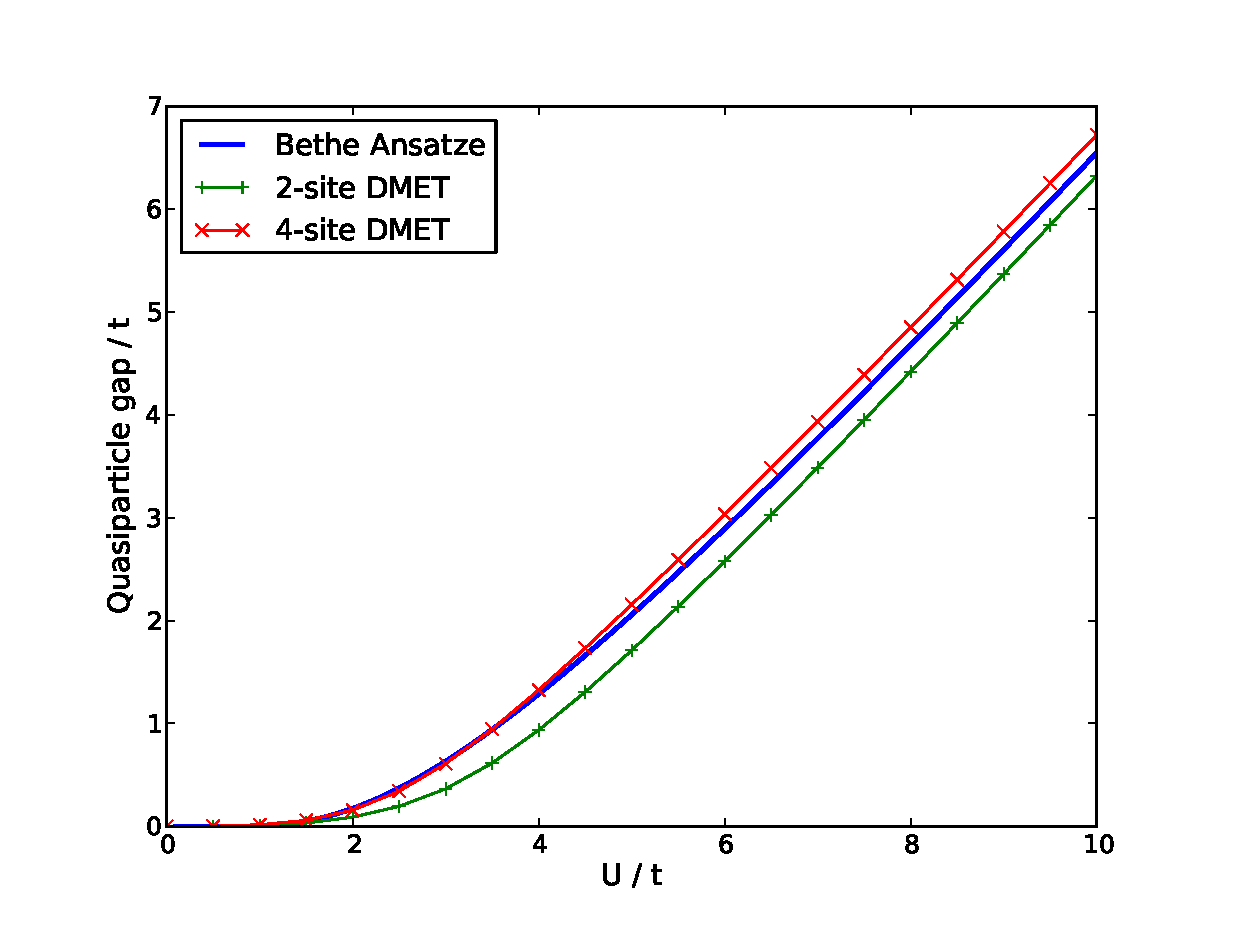
\includegraphics[scale=0.475]{Plots/1D_Gap/Hubbard_Gap.eps}
\end{center}
    \vspace{-8mm}
\caption{Error in the spectral gap from the 1-particle and 2-particle greens functions compared to analytic results
from the Bethe Ansatze\cite{Ovchinni1970}, and six bath orbital CDMFT results\cite{Go2009}. The convergence of the
DMET results with increasing cluster size is shown.}
\label{1D_GAP}
\end{figure}

{\emph Results.-} We first examine the one-dimensional Hubbard model, whose ground state energy\cite{Lieb68} and spectral gap\cite{Ovchinni1970} are analytically Bethe-Ansatz solvable, and additionally compare to
zero-temperature, large cluster-DMFT results\cite{Go2009}. Figure~\ref{1D_DOS} shows the local density of states, calculated with a four-site impurity cluster, and compared to six-site
cluster-DMFT results, obtained via an exact diagonalization within six bath orbital representation of the continuum, as found in Ref.~\onlinecite{Go2009}. Since exact diagonalization was used as the impurity solver, 
the spectra are obtained on the real axis at zero-temperature, and so can be directly compared against. As expected in the one-dimensional case, there is no
frustration, and the system is dominated at all values of $U$ by long-range magnetic ordering\cite{Lieb68}. Consequently, there is no Mott transition and the system is insulating for arbitrarily small values of $U$,
in both the DMET and CDMFT spectra. 

Although the qualitative aspects of the spectral gap are well reproduced between the two methods, the higher frequency excitations in the CDMFT calculations are very noisy, which makes it difficult to determine 
which features are physical, and which are spurious and a result of the finite (six) bath representation of the coupling of the cluster to the environment. In contrast, the DMET results give an entirely smooth
representation of the spectra, due to the analytic construction of the exact coupling to $|\phi^{(1)}(\omega)\rangle$ at each frequency. However, at very high frequencies, outside the bandwidth of the 
$|\phi^{(1)}(\omega)\rangle$, there is little or no coupling of the local excitation spectrum to the environment provided by the bath construction and so the uncoupled local excitations result. 
Therefore, in the results presented, the spectral window probed will be determined by the bandwidth of $|\phi^{(1)}(\omega)\rangle$. Another point to note is that the sum rules on the spectral functions are
exactly obeyed, and the integrated spectral weight of the results in Fig.~\ref{1D_DOS} are all unity.
For comparison, Fig.~\ref{1D_GAP} shows the error in the spectral gap to the analytic result\cite{Ovchinni1970}, demonstrating the convergence towards the exact spectral gap as the cluster size is increased 
from two to four sites, and indicating a generally similar quality of results to CDMFT calculations of the same cluster size.

%+++++++++++++++++++++++++++++++++++++++++++++++++++++++
%   DD response 
%+++++++++++++++++++++++++++++++++++++++++++++++++++++++
\begin{figure}
\begin{center}
    \vspace{-2mm}
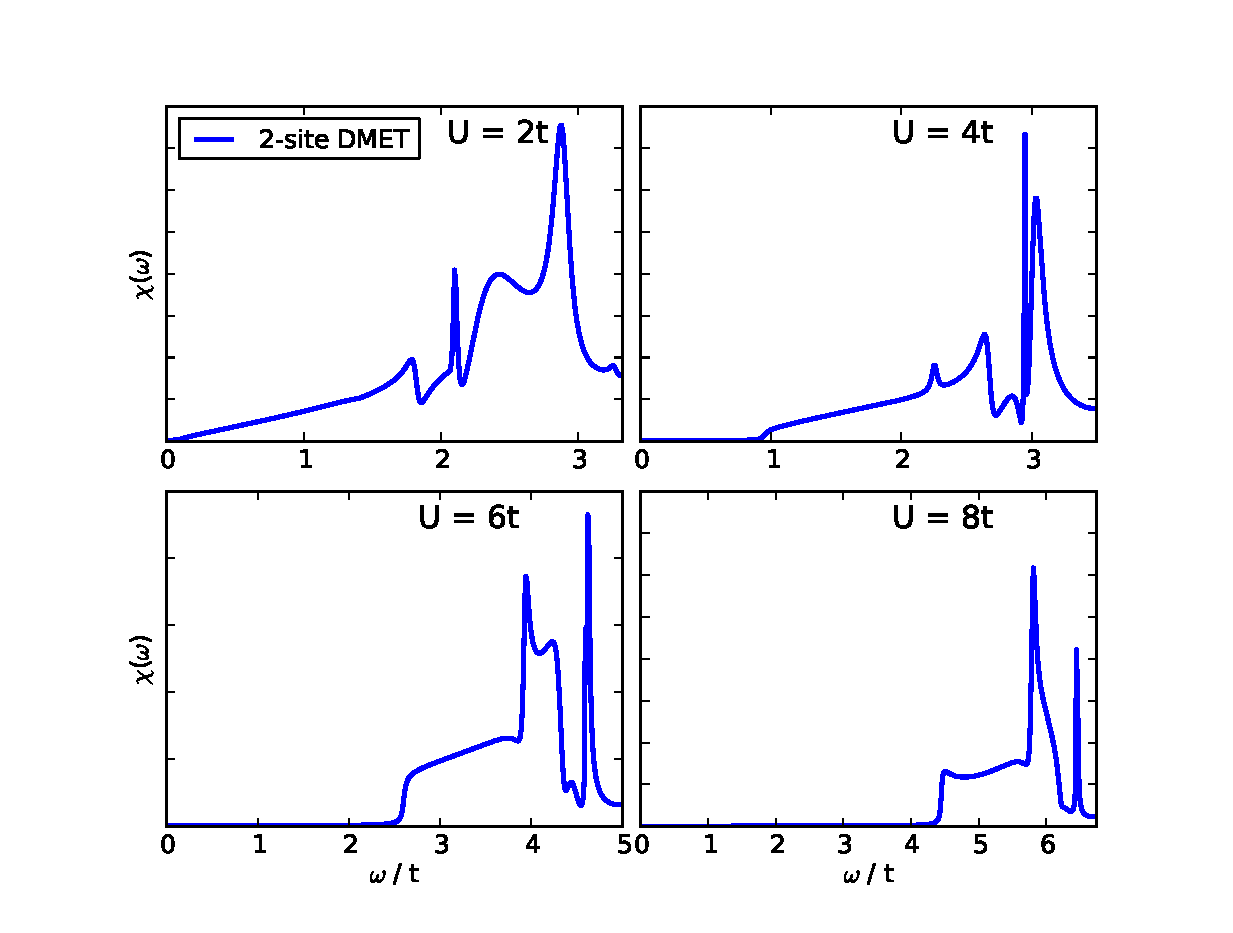
\includegraphics[scale=0.475]{Plots/1D_DD/1D_Hub_DD.eps}
\end{center}
    \vspace{-8mm}
\caption{Two impurity DMET calculation of the local density-density response function for the half-filled 1D Hubbard model via construction of the 2-particle greens function.
The spectral gap is used in the data plotted in Fig.~\ref{1D_GAP}}
\label{1D_DD}
\end{figure}

Fig.~\ref{1D_DD} shows the local density-density response function of the 1D Hubbard model at half-filling, obtained from the local two-particle Greens 
function (${\hat V}={\hat A}=a_{\alpha}^{\dagger}a_{\alpha}$). The poles of this function correspond to the neutral excitation energies, and as such determine 
many of the optical properties of the system\cite{Millis2012,Essler91}.
Unfortunately, direct comparison of the spectra in Fig.~\ref{1D_DD} to other methods is difficult due to the paucity of other comparable methods for this important quantity.
However, since long-range correlations are not included in the Hubbard Hamiltonian, 
%exciton binding is negligable, and 
the optical and quasiparticle gaps obtained from system should be the same. The excitation gaps
obtained from the two-particle Greens functions are included in Fig.~\ref{1D_GAP}, and show that for the same cluster size, the differences between the spectral gaps are negligible 
on the scale of the plot. However, while not conclusive, this supports the assertion that the one- and two-particle Greens functions are of similar quality, while also of comparable computational cost.

%+++++++++++++++++++++++++++++++++++++++++++++++++++++++
%   2D HUBBARD PLOTS 
%+++++++++++++++++++++++++++++++++++++++++++++++++++++++
\begin{figure}
\begin{center}
    \vspace{-2mm}
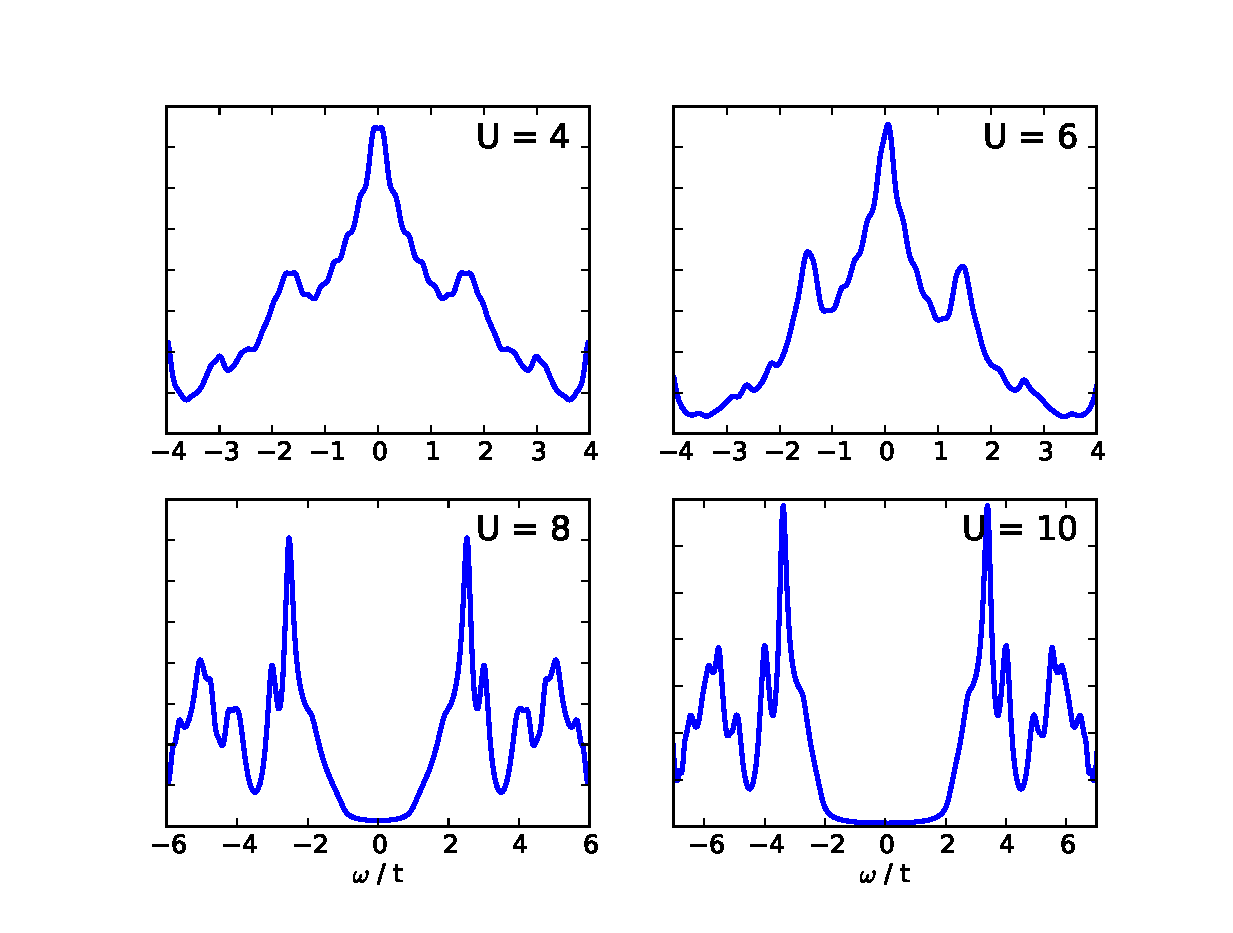
\includegraphics[scale=0.475]{Plots/2D_Spectra/2DHub_Spectra.eps}
\end{center}
    \vspace{-8mm}
\caption{Local density of states of the half-filled 2D Hubbard model from a $2 \times 2$ impurity cluster DMET calculation, showing a MIT at $U\approx5.5t$}
\label{2D_DOS}
\end{figure}


%+++++++++++++++++++++++++++++++++++++++++++++++++++++++
%   2D DOPED HUBBARD PLOTS 
%+++++++++++++++++++++++++++++++++++++++++++++++++++++++
\begin{figure}
\begin{center}
    \vspace{-2mm}
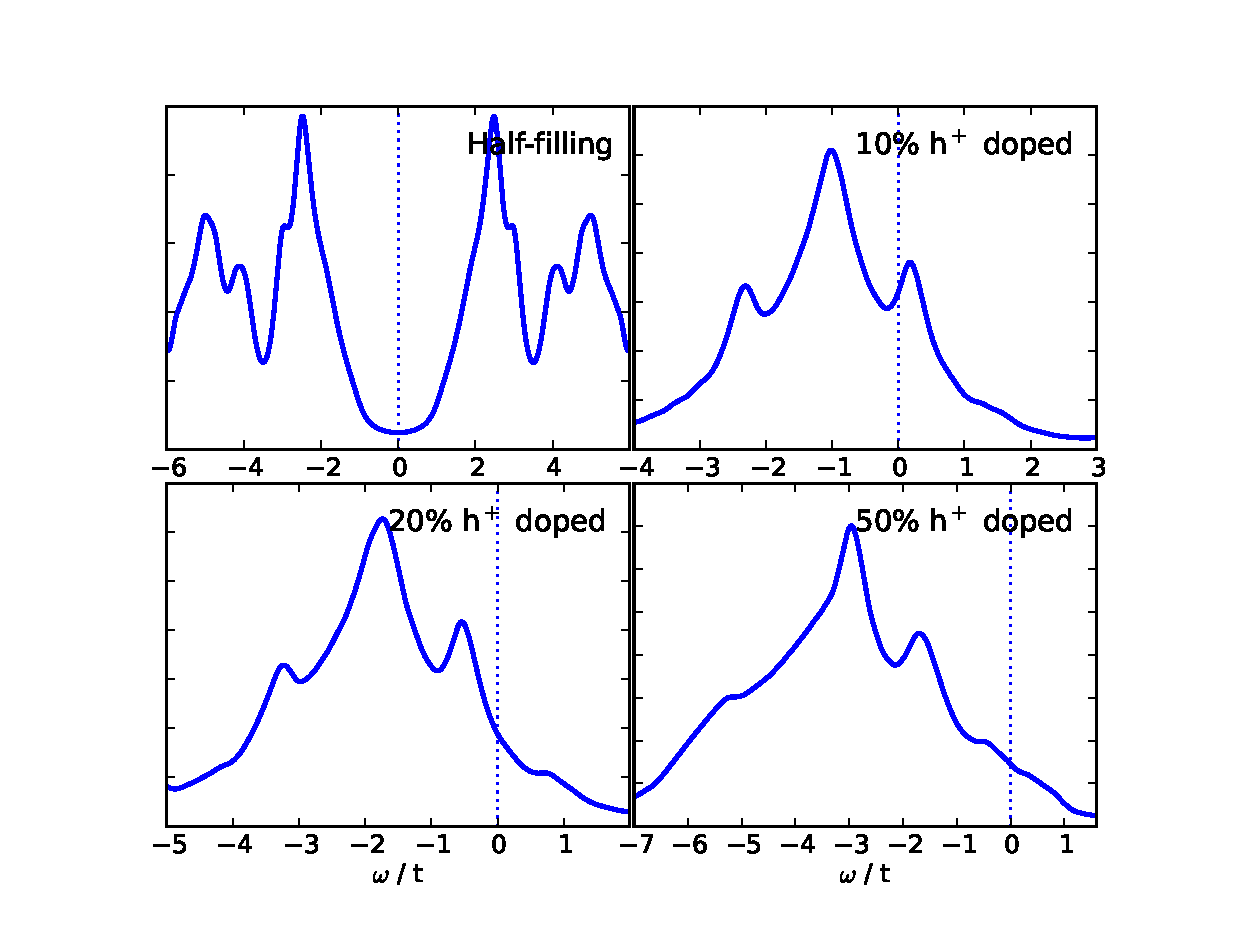
\includegraphics[scale=0.475]{Plots/Doping/2D/nImp4/U8/LargerBroadening/2DHub_Doping.eps}
\end{center}
    \vspace{-8mm}
\caption{Local density of states of the hole doped 2D Hubbard model calculated with a four impurity cluster with $U = 8t$.}
\label{2D_Doped}
\end{figure}

A sterner test comes from the 2D Hubbard model in the paramagnetic phase, which still receives widespread attention in the condensed matter community\cite{Georges1996,Senechal2000,Kotliar2008,Millis2012,Millis2013}
due to its first-order metal-insulator transition (MIT) arising from competing magnetic effects as the correlation strength, $U$, is increased. The DMET local density of
states are shown in Fig.~\ref{2D_DOS}, for a $2 \times 2$ plaquette of impurity sites. In the low $U$ regime, the famous `three-peak' structure is observed, with a central 
Kondo resonance peak, and the Hubbard bands either side. At $U \approx 6.9t$, there is a transition to an insulating regime, with a Mott gap opening with increased
$U$. The spectra then feature prominent coherence peaks at the gap edge, as have been observed elsewhere. Cluster DMFT calculations with the same plaquette
size observe a MIT at a slightly lower $U\approx5.5t$, with a coexistance region at low temperatures, which we also observe\cite{Kotliar2008}. However, analytically continued
spectral functions from CT-QMC smooth out many of the subtle correlation driven substructures observed in Fig.~\ref{2D_DOS}. Fig.~\ref{2D_Doped} shows the effect on the 
spectra upon hole doping the system, which is shown for the insulating phase at $U=8t$. Once doped, the system returns to a Fermi liquid phase, and 
particle-hole symmetry is broken.

In conclusion, we have presented a quantum embedding formulation for accurate, zero-temperature spectral functions of extended correlated systems at a small computational cost, which vastly 
extends the scope of the DMET method. The approach has a number of 
advantageous formal properties. 
\begin{inparaenum}[\itshape i\upshape)]
\item The embedding within the environment is achieved via coupling to a small set of analytically constructed, many-electron bath states,
    which are derived from the formal Schmidt decomposition of the response vector obtained from a one-electron Hamiltonian. The coupling therefore exactly spans this vector, and
    changes with frequency, to give smooth spectra without any error from the discretization of the continuum
\item Spectral functions are obtained on the real frequency axis, removing the need for any analytic continuation from the imaginary axis
\item The calculation of the interacting problem is performed in a basis that is independent of the size of the underlying lattice, and which is constructed in a cost no greater than the
    diagonalization of the one-electron Hamiltonian
\item Both extension to clusters of impurity sites, and arbitrary perturbation rank are straightforward within the framework.
\end{inparaenum}
The approach was demonstrated on the one- and two-dimensional Hubbard model, and compared favorably to both exact results and cluster DMFT calculations. Extensions are now underway for the
calculation of non-local operators, an {\em ab initio} formulation, and for the investigation of different phases by embedding within broken symmetry mean-field Hamiltonians.

\bibliography{SpectralDMETBib}

\end{document}
